\documentclass[11pt, letterpaper]{article}
\usepackage[utf8]{inputenc}
\usepackage[english]{babel}
\usepackage[margin=1in]{geometry}
\usepackage{indentfirst}
\usepackage{titling}
\usepackage{graphicx}
\usepackage{amsmath}
\usepackage{hyperref}
\graphicspath{ {./} }

\setlength{\parindent}{0cm}
\setlength{\parskip}{1em}
\renewcommand{\baselinestretch}{1.5}

\hypersetup{
    colorlinks=true,
    linkcolor=cyan,
    filecolor=magenta,      
    urlcolor=blue,
}

\title{Chapter I: Fields}
\author{Chenyi Zhu}
\date{Jan 13th, 2020}

\begin{document}

\begin{titlingpage}

		\maketitle
		%\begin{abstract}
			%From Physics I: Classical Mechanics we were introduced to gravity and the 
			%gravitational field. Now for Physics II: Electromagnetism, we will be working
			%with electrical and magnetic fields. They may sound daunting in the beginning,
			%but soon you will see that they are very similar to the concepts we have seen
			%when studying gravity. \par
			
			\begin{figure}[h!]
				\centering
				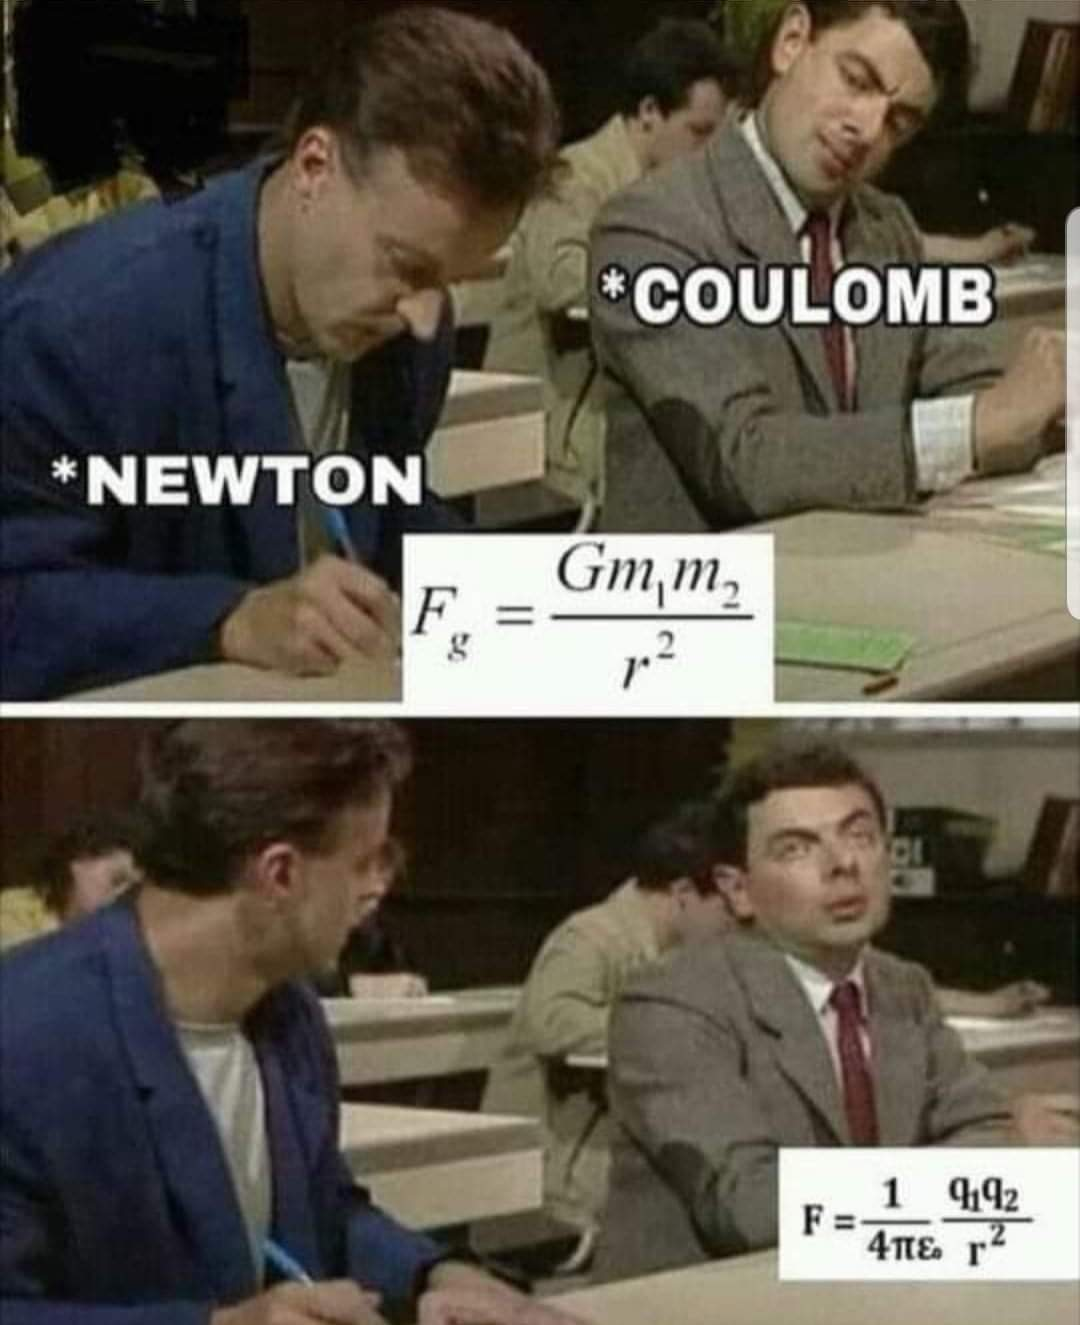
\includegraphics[scale=0.2]{coulomb.jpg}
				\label{fig:coulomb-meme}
			\end{figure}
			
		%\end{abstract}
		
\end{titlingpage}

\section{Gravitational Field.}

		\begin{figure}[h!]
			\centering
			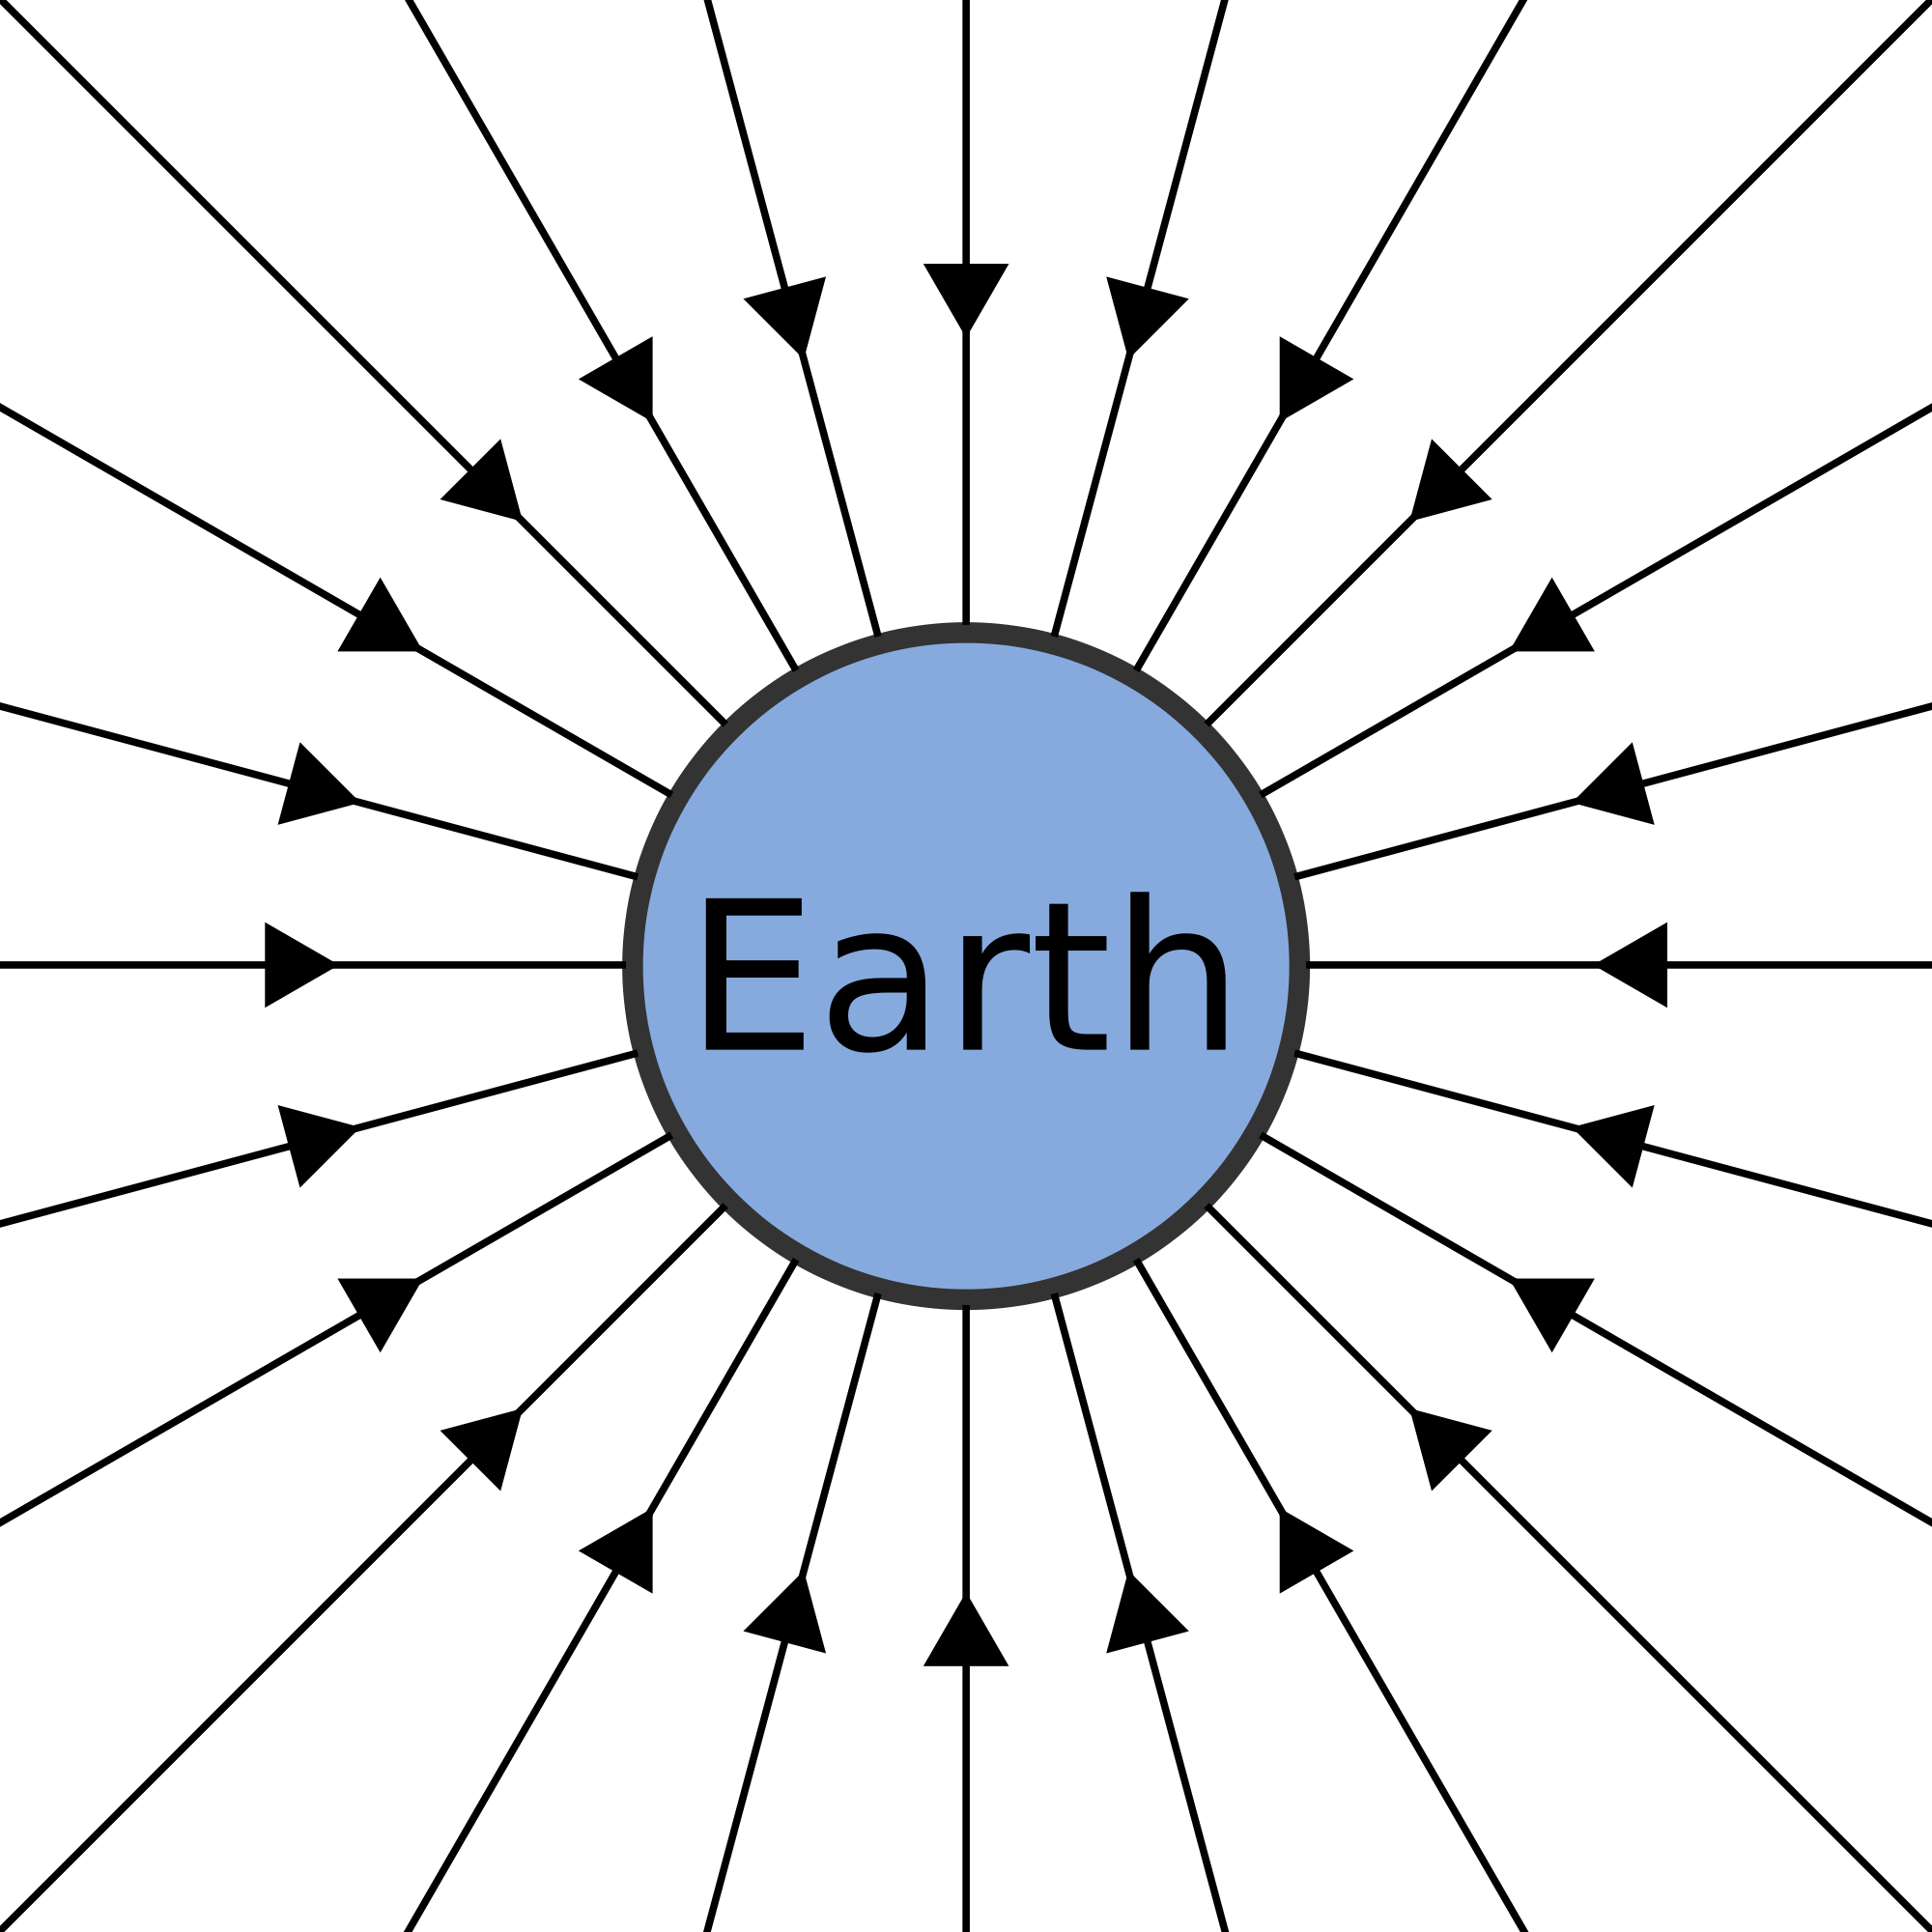
\includegraphics[scale=0.03]{gravitational-field}
			\caption{\href{https://www.tes.com/lessons/Z-xymdzS_E4_uQ/g484-chapter-4-
			gravitational-fields}{Earth's gravitational field lines}.}
			\label{fig:gravity}
		\end{figure}
		
		Gravitational force is defined as:
		\begin{equation}\label{eqn:gravi-force}
			\boxed{\vec{F_g} \equiv -G\frac{Mm}{r^2}\,\hat{r}}
		\end{equation}
		from which we can easily derive the gravitational field by setting m to be 
		negligible:
		\begin{equation}\label{eqn:gravi-field}		
			\boxed{\vec{g} \equiv \displaystyle\lim_{m \to 0} \frac{\vec{F_g}}{m} = 
			-G\frac{M}{r^2}\,\hat{r}}
		\end{equation}
		
		\noindent\textbf{Note}: Near earth's surface, gravitational field $\vec{g}$ is approximately
		constant.
				\[\vec{g} \equiv -g\,\hat{r} \qquad \text{where} \qquad g \equiv G\frac{M}{R_E^2}\approx
				9.8\,m/s^2\]
		 A mass in constant gravitational field (e.g. near Earth's surface) doesn't
		necessarily move in the direction of the field unless initial velocity moves in the same
		direction. If initial velocity is perpendicular to the direction of the field, the trajectory will 
		be parabolic.

\section{Electric Field.}	

		\begin{figure}[h!]
			\centering
			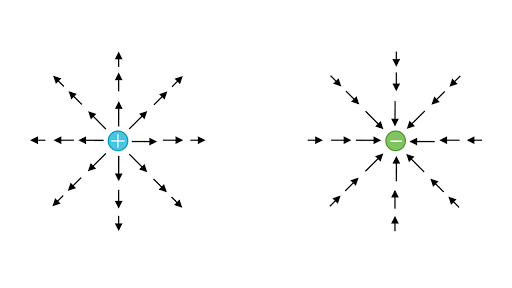
\includegraphics[scale=0.33]{electric-field}
			\caption{\href{https://www.khanacademy.org/science/electrical-engineering/ee-
			electrostatics/ee-electric-force-and-electric-field/a/ee-electric-field}{Electric field 
			lines of positive and negatively charged particles}.}
			\label{fig:electric}
		\end{figure}
	
		Force due to an electric field is called \textbf{Coulomb's force}, which is defined here as:
		\begin{equation}\label{eqn:coulomb-force}
			\boxed{\vec{F_e} \equiv k_e \frac{Qq}{r^2}\,\hat{r}}
		\end{equation}
		and we now observe lots of similarity between the forms of the two different fields. Taking
		the limit as before and we observe:
		\begin{equation}\label{eqn:electric-field}
			\boxed{\vec{E} \equiv \displaystyle\lim_{q \to 0} \frac{\vec{F_e}}{q} = k_e\frac{Q}{r^2
			}\,\hat{r}}
		\end{equation}
		
		Now we get a grasp of the link between gravity and electricity. You now know that electric 
		force arises when two or more charged particles interact with each other, and 
		a single charged particle produces its own electric field (recall: you can think of the 
		gravitational field as being produced by a single mass, which bends space and time). The 
		main difference here (other than the constants in the equations) is that gravitational force is 
		\textbf{ALWAYS} attractive, while electric force can be \textbf{EITHER} attractive or repulsive.
		
\section{Magnetic Field.}


		Magnetic field is a very special member of this family. It is a little more complex than the 
		other two, and I will not go into the equations just yet. However, I would like to illustrate why 
		it is considered "special".
		
		\begin{figure}[h!]
			\centering
			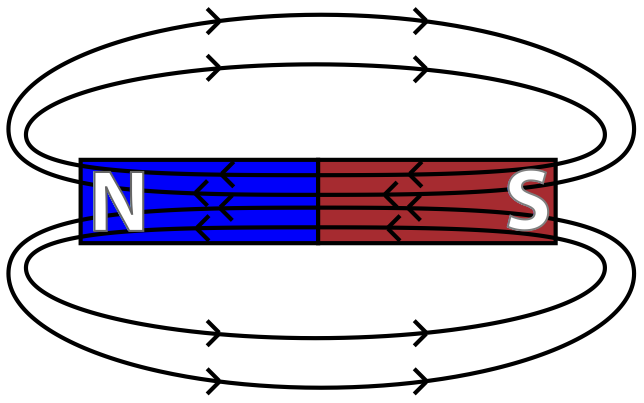
\includegraphics[scale=0.5]{magnetic-field-lines}
			\caption{\href{https://www.aplusphysics.com/courses/honors/magnets/magfields.html}
			{Magnetic field lines}.}
			\label{fig:magnetic}
		\end{figure}
		
		Simply based on the picture above, we can see a magnet which produces magnetic field 
		going from the North to the South pole. Interesting observation: in the past, we have 
		been saying that we need at least two masses or charged particles to produce a
		field. Here, however, we only need one magnet to produce a field. There are no such thing
		as a \textbf{monopole} in magnetism, but only \textbf{dipole}, and you will learn more about 
		this special identity later on in this course. 


\end{document}
